\documentclass[11pt]{ctexart}

\usepackage{amsmath}
\usepackage{amssymb}
\usepackage{bm}

\usepackage{algorithm}
\usepackage{algorithmic}

\usepackage{graphicx}

\title{ \textbf{生成式对抗网络(GAN)的原理和各种变种类型的介绍} }
\author{C. Lu}


\begin{document}
\maketitle

\section{生成式对抗网络}
\subsection{引言}
\emph{生成式对抗网络}(generative adversarial network, GAN)\cite{goodfellow2014generative} 是基于可微生成器网络的一种生成式数据建模方法。

生成式对抗网络基于博弈论场景,其中生成器网络必须与对手竞争。生成器网络直接产生样本$\bm x = g(\bm z; \bm \theta^{(g)})$。其对手,\emph{判别器网络}(discriminator network)试图区分从训练数据抽取的样本和生成器中抽取的样本。判别器发出由$d(\bm x; \bm \theta^{(d)})$给出的概率值,指示$\bm x$是真实训练样本而不是从模型中抽取的伪造样本的概率, GAN的结构如图\ref{gan}。

\begin{figure}[htbp]
	\centering
	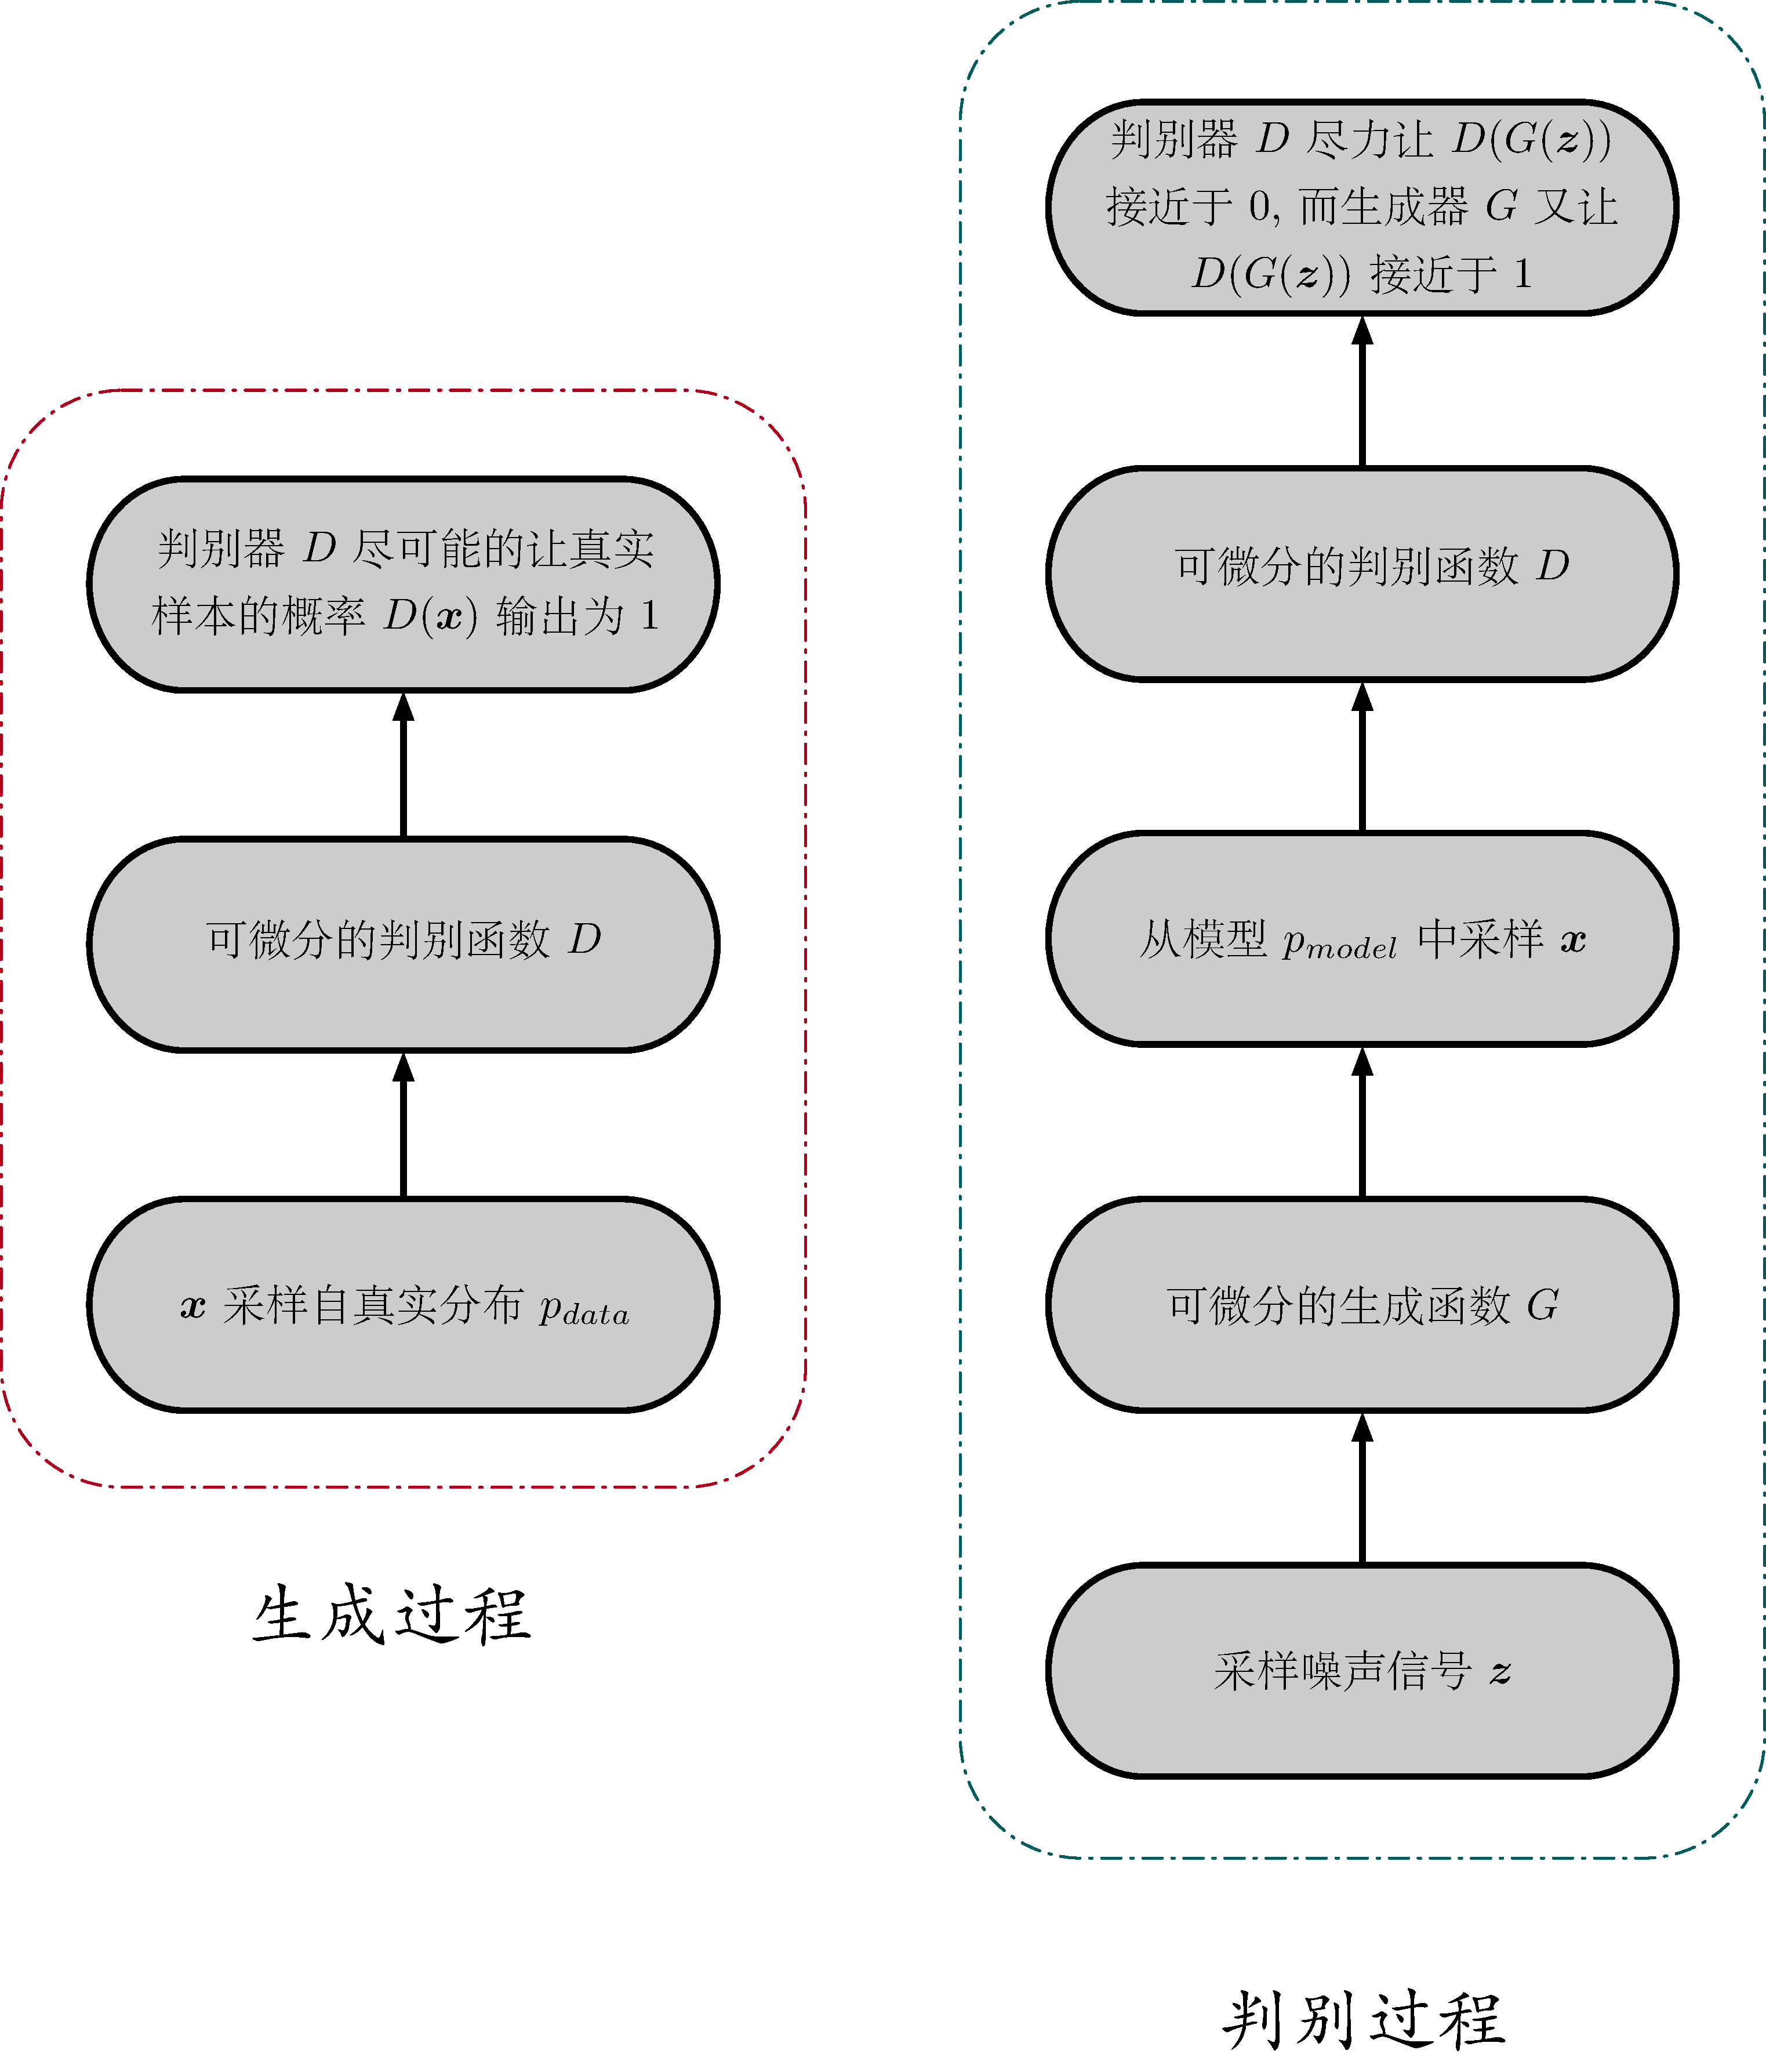
\includegraphics[width=6cm]{GAN}
	\label{gan}
	\caption{GAN的结构示意图}
\end{figure}

形式化表示生成式对抗网络中学习的最简单的方式是零和游戏,其中$v(\bm\theta^{(g)}, \bm\theta^{(d)})$确定判别器的收益。生成器接收$-v(\bm\theta^{(g)}, \bm\theta^{(d)})$作为它自己的收益。在学习期间,每个玩家尝试最大化自己的收益,因此收敛在
	\begin{equation}
	\label{eq:minimax}
		g^* = \arg \min_{g} \max_{d} \ v(g, d)
	\end{equation}		
$v$的默认选择是
	\begin{equation}
		v(\bm \theta^{(g)}, \bm \theta^{(d)}) = \mathbb{E}_{\bm x\sim p_{\mathrm{data}}}\log d(\bm x) + \mathbb{E}_{\bm x\sim p_{\mathrm{model}}}\log(1-d(\bm x))
	\end{equation}
	这驱使判别器试图学习将样品正确地分类为真的或者伪造的。同时,生成器试图欺骗分类器以让其相信样本是真实的。在收敛时,生成器的样本与实际数据不可区分,并且判别器处处都输出$\frac{1}{2}$。然后就可以丢弃判别器。
	
	设计GAN的主要动机是学习过程既不需要近似推断,也不需要配分函数梯度的近似。当$\max_{d}v(g,d)$在$\bm\theta^{(g)}$中时凸的(例如,在概率密度函数的空间中直接执行优化的情况)时,该过程保证收敛并且是渐近一致的。
\subsection{生成式对抗网络的训练算法}
	生成式对抗网络的训练式生成器与判别器互相博弈的过程。生成器与判别器交替使用最优化算法(如:梯度下降算法)来最大化各自的价值函数。在训练初期,判别器的能力较弱,无法正确区分出真实样本和伪造样本;此时,可以认为设立一个超参数	$k$, 训练$k$轮判别器后,再进行生成器的训练。具体算法流程如算法\ref{alg:gan}所示。
	\begin{algorithm}
		\caption{生成式对抗网络的随机梯度下降训练算法。判别器训练的循环次数$k$是人为指定的超参数。($k\geq 1$) }
		\label{alg:gan}
		\begin{algorithmic}[1]
		\FOR {训练迭代次数}
			\FOR {$k$}
				\STATE 从噪声的先验分布$p_g(\bm z)$中采样$m$个噪声样本$\{\bm z^{(1)}, \bm z^{(2)}, \ldots,\bm  z^{(m)}\}$
				\STATE 从数据的真实分布$p_{\mathrm{data}}(\bm x)$中采样$m$个真实数据样本 $\{\bm x^{(1)}, \bm x^{(2)}, \ldots, \bm x^{(m)}\}$
				\STATE 通过梯度上升法来更新判别器的参数,梯度由以下公式给出:
						\[
						\nabla_{\bm \theta_d}\frac{1}{m} \sum_{i=1}^{m}\left[\log D\left(\bm x^{(i)}\right) + \log\left(1-D\left(G\left(\bm z^{(i)}\right)\right)\right)\right]
						\]
			\ENDFOR	
			
			\STATE 从噪声的先验分布$p_g(\bm z)$中采样$m$个噪声样本$\{\bm z^{(1)}, \bm z^{(2)}, \ldots,\bm  z^{(m)}\}$
			\STATE 通过梯度下降法来更新判别器的参数,梯度由以下公式给出
					\[
						\nabla_{\bm \theta_g}\frac{1}{m} \sum_{i=1}^{m}\left[ \log\left(1-D\left(G\left(\bm z^{(i)}\right)\right)\right)\right]
						\]
		\ENDFOR
		\end{algorithmic}
	\end{algorithm}

\subsection{生成式对抗网络的理论依据}
\cite{goodfellow2014generative}中证明了式(\ref{eq:minimax})的最优解为
	\[
		p_g = p_{data}
	\]
即生成模型能够很好的代表了真实数据的分布。
	
\section{深度卷积生成式对抗网络}
在实践中,由神经网络表示的$g$和$d$以及$\max_dv(g,d)$不凸时,GAN中的学习可能是困难的。\cite{goodfellow2014distinguishability}认为不收敛可能会引起GAN的欠拟合问题。稳定的GAN学习仍然是一个开放问题。幸运的是,当仔细选择模型架构和超参数时,GAN的学习效果很好。\cite{radford2015unsupervised}设计了一个\emph{深度卷积生成式对抗网络}(DCGAN),在图像合成的任务上表现非常好,并表明其潜在的表示空间能捕获到变化的重要因素。图\ref{fig:face} 展示了生成器生成的图像实例。

\begin{figure}[htbp]
\centering
\begin{minipage}[t]{0.48\textwidth}
\centering
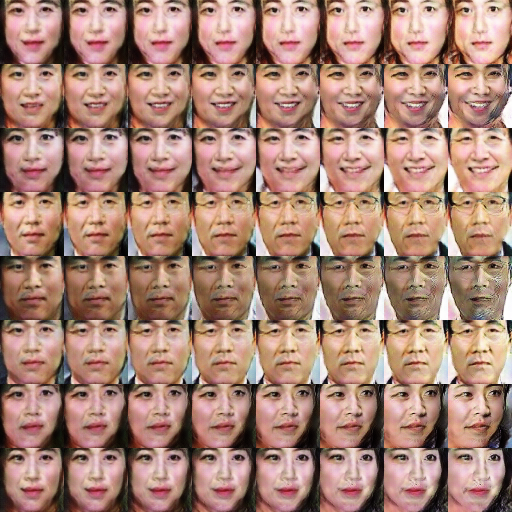
\includegraphics[width=4cm]{asia_face}
\label{fig:face}
\end{minipage}
\begin{minipage}[t]{0.48\textwidth}
\centering
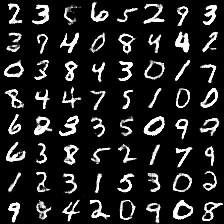
\includegraphics[width=4cm]{mnist}
\label{fig:mnist}
\end{minipage}
\caption{在亚洲人脸数据集(左)和手写数字数据集(右)上训练后,由DCGAN生成的图像}
\end{figure}

\subsection{深度卷积生成式对抗网络架构}
深度卷积生成式对抗网络(DCGAN)采用卷积神经网络(CNN)作为生成器和判别器。与原始的CNN架构不同,DCGAN主要做了以下几点重要的改动:
\begin{description}
	\item[\emph{移除池化函数}]将所有的池化函数(如:MaxPooling)全部替换为固定步长的卷积函数。这样做的目标是为了让神经网络自己去学习如何采样。
	\item[\emph{移除全连接层}] 移除CNN中的全连接层。对于判别器来说,最后一层卷积输出被展平成一个向量;对于生成器,噪声信号$\bm z$采样自一个均匀分布,乘以一个变换矩阵$\bm W$之后变成一个高维向量,然后将其重新调整为一个$4$维的张量。具体结构如图\ref{fig:dcgan}所示。
	\item[\emph{批标准化}] 在生成器与判别器的网络中加入\emph{批标准化层}\cite{ioffe2015batch}。批标准化是一个自适应的重参数化的方法,可以用来训练非常深的模型。如果直接将批标准化应用到模型的每一层中,会导致生成样本和模型的不稳定性,所以,在DCGAN中,生成器的输出层和判别器的输入层没有加入批标准化。
	\item[\emph{激活函数的改动}] 生成器中使用ReLU\cite{nair2010rectified} 激活函数,输出层是用 Tanh激活函数;与原始GAN使用的Maxout\cite{goodfellow2013maxout} 激活函数不同,判别器使用LeakyReLU\cite{xu2015empirical} 会有更好的效果,而且在更深的模型效果更显著。
\end{description}

\begin{figure}[htbp]
	\centering
	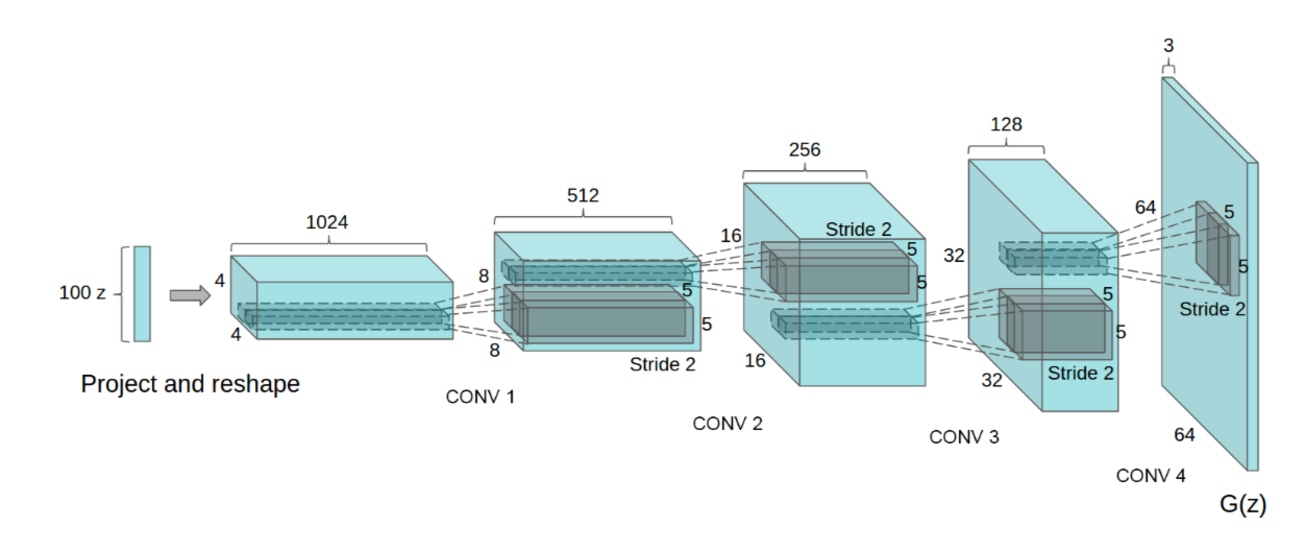
\includegraphics[width=10cm]{DCGAN}
	\label{fig:dcgan}
	\caption{用于LSUN数据集的DCGAN生成器的结构示意图}
\end{figure}


\subsection{DCGAN中特征表示的向量运算}
生成器从采样噪声$\bm z$中经过卷积运算生成特定的图像样本,可以把噪声信号$\bm z$认为是生成图片的低维表示,$\bm z$的每个分量代表图像的某种特征。例如,对于人脸图像,$\bm z$的某个分量代表了性别,其他某个分量代表了是否带眼镜。与\emph{词向量}类似,可以进行算数上的加减操作,如:
	\[
		\bm v(\text{国王}) - \bm v(\text{男人}) + \bm v(\text{女人}) = \bm v(\text{王后})
	\]
\cite{radford2015unsupervised}中给出了类似的实验结果,如图\ref{fig:dcgan2} 所示。
\begin{figure}[H]
	\centering
	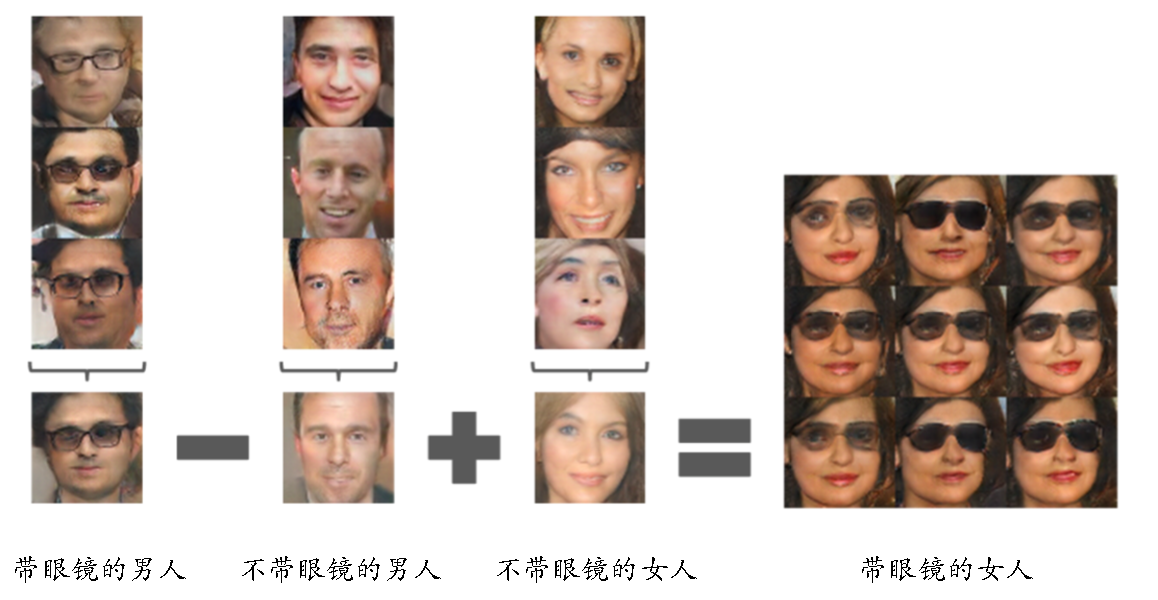
\includegraphics[width=10cm]{dcgan2}
	\caption{CGAN中特征表示的向量运算}
	\label{fig:dcgan2}
\end{figure}


\section{条件生成式对抗网络}
\emph{条件生成式对抗网络}(Conditional GAN, 简称CGAN)
是在原始生成式对抗网络的生成器和判别器中都加入条件信息$\bm y$,(例如,在手写数字识别的问题中,$\bm y$可能是特定的数字标签;在图像生成的问题中,$\bm y$可以是对要生成图像的特定描述),控制生成模型生成满足特定条件的样本。

在原始GAN的生成器中,输入的噪声信号$\bm z$带代表了要生成图像的低维表示;同样的,也可以将要加入的附加信息进行编码,得到附加信息的向量表示$\bm y$, 之后,将$\bm z$与 $\bm y$一同输入到生成器中,以产生特定条件限制下的样本。对于判别器也是类似的操作,同时将样本$\bm x$(来自真实分布$p_{data}$或者模型的分布$p_{model}$)与条件信息$\bm y$输入进行判别。

条件生成式对抗网络的目标函数如公式\ref{eq:cgan}所示:
\begin{equation}
\label{eq:cgan}
	V(\bm \theta^{(G)}, \bm \theta^{(D)}) = \mathbb{E}_{\bm x\sim p_{\mathrm{data}}}\log D\left(\bm x | \bm y\right) + \mathbb{E}_{\bm z\sim p_{\bm z}\left(\bm z\right)}\left[\log\left(1-D\left(G\left(\bm z|\bm y\right)\right)\right)\right]
\end{equation}
图\ref{fig:cgan}简要的展示的使用神经网络的条件生成对抗网络。
\begin{figure}
	\centering
	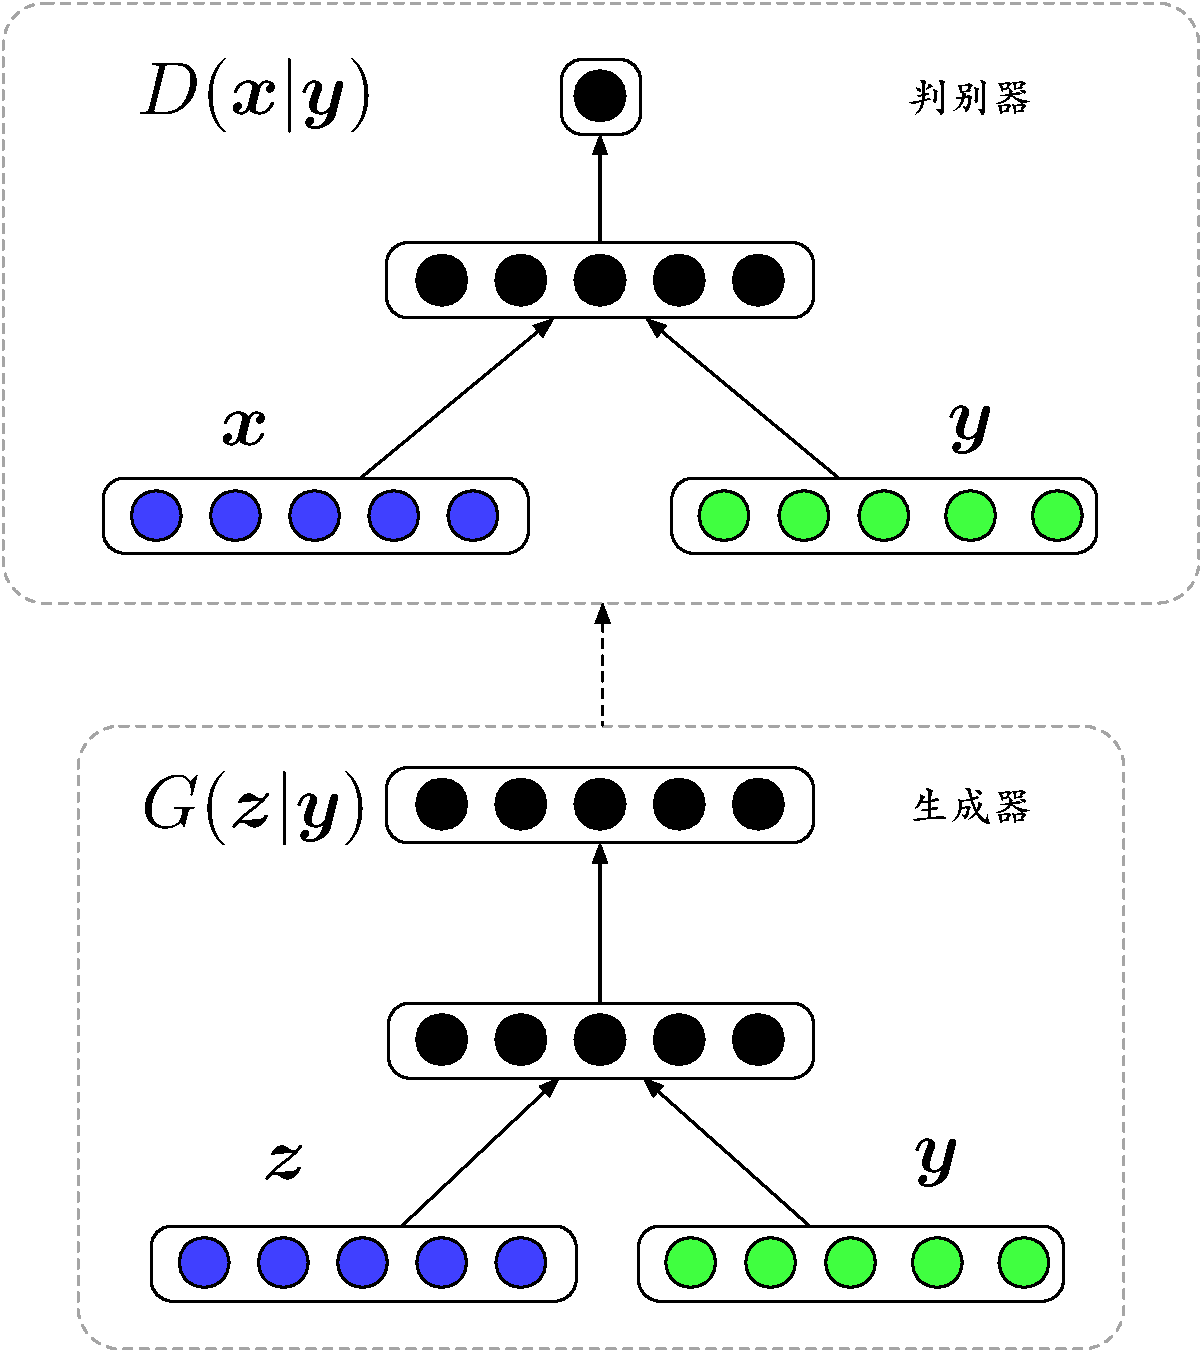
\includegraphics[width=6cm]{CGAN}
	\label{fig:cgan}
	\caption{条件生成对抗网络}
\end{figure}

\subsection{条件生成对抗网络的实例}
\subsubsection{手写数字生成}


\subsubsection{基于多模态的图像自动标注}
\subsection{条件对抗网络之图像到图像的转换}


\section{基于能量的生成式对抗网络}
\newpage
\bibliographystyle{plain}
\nocite{*}
\bibliography{reference}

\end{document}

